%%%%%%%%%%%%%%%%%%%%%%%%%%%%%%%%%%%%%%%%%%%%%%%%%%%%%%%%%%%%%%%%%%%%%%%%%%%%%%%%%%%%%%%%%%%%%%%%%%%%%%%%%%%%%%%%%%%%%%%%%%%%%%%%%%%%%%%%%%%%%%%%%%%%%%
% 20141002 - Introduction to Operating Systems VO
%%%%%%%%%%%%%%%%%%%%%%%%%%%%%%%%%%%%%%%%%%%%%%%%%%%%%%%%%%%%%%%%%%%%%%%%%%%%%%%%%%%%%%%%%%%%%%%%%%%%%%%%%%%%%%%%%%%%%%%%%%%%%%%%%%%%%%%%%%%%%%%%%%%%%%

\tikzstyle{block} = [rectangle, draw, fill=blue!20, 
    text width=10em, text centered, rounded corners, minimum height=3em]
\tikzstyle{info} = [rectangle, draw, 
    text width=10em, text centered, rounded corners, minimum height=3em]

%fancyhdr
\lhead{IOS VO} 
\rhead{2014-10-02}

%%%%%%%%%%%%%%%%%%%%%%%%%%%%%%%%%%%%%%%%%%%%%%%%%%%%%%%%%%%%%%%%%%%%%%%%%%%%%%%%%%%%%%%%%%%%%%%%%%%%%%%%%%%%%%%%%%%%%%%%%%%%%%%%%%%%%%%%%%%%%%%%%%%%%%

\section*{Architecture}

%%%%%%%%%%%%%%%%%%%%%%%%%%%%%%%%%%%%%%%%%%%%%%%%%%%%%%%%%%%%%%%%%%%%%%%%%%%%%%%%%%%%%%%%%%%%%%%%%%%%%%%%%%%%%%%%%%%%%%%%%%%%%%%%%%%%%%%%%%%%%%%%%%%%%%

\par{
	\begin{figure}[H]
		\centering
		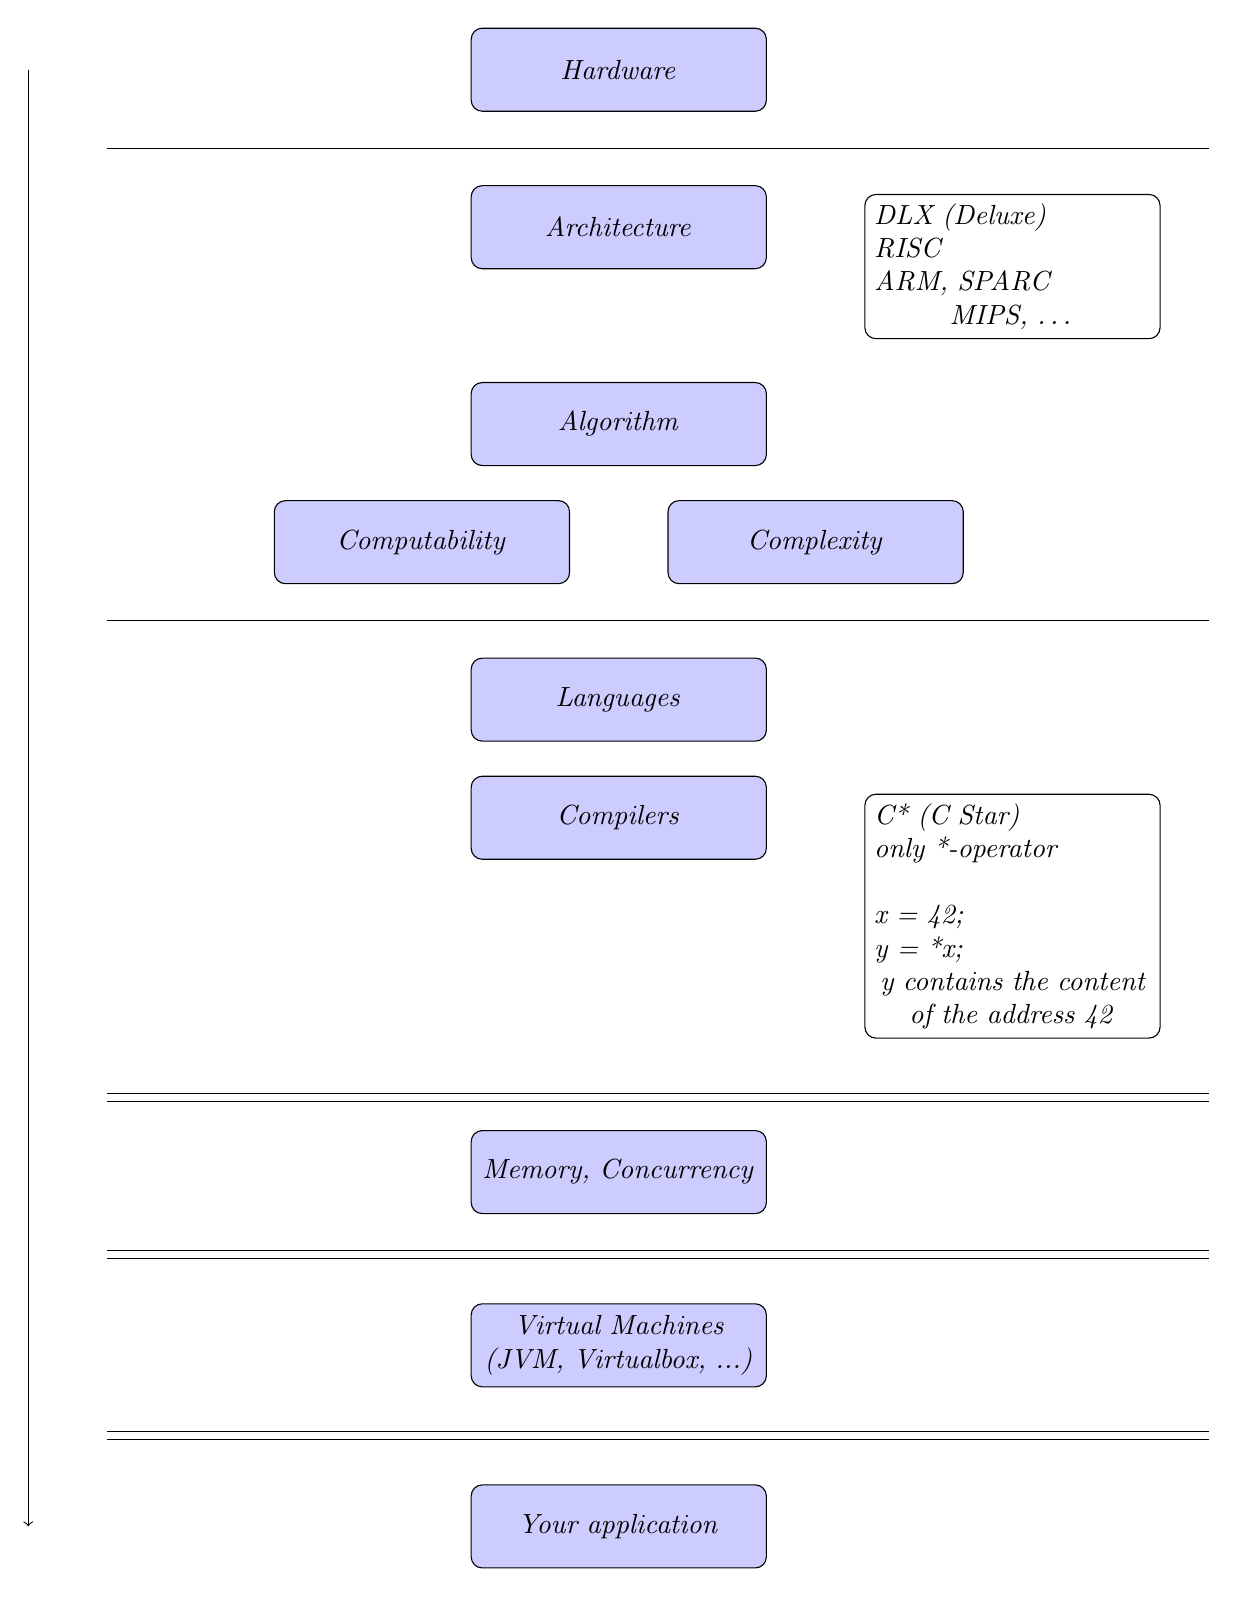
\begin{tikzpicture}[scale = 1.0]
			\draw[->] (0, 20) -- (0, 1.5);

			\node[block] (hardware) at (7.5, 20) {\textit{Hardware}};
            \draw (1, 19) -- (15, 19);
            
            \node[block] (architecture) at (7.5, 18) {\textit{Architecture}};
            \node[info] (archictectureinfo) at (12.5, 17.5) {\textit{DLX (Deluxe) \newline RISC \newline ARM, SPARC \newline MIPS, \ldots}};

            \node[block] (algorithm) at (7.5, 15.5) {\textit{Algorithm}};
            \node[block] (computability) at (5, 14) {\textit{Computability}};
            \node[block] (complexity) at (10, 14) {\textit{Complexity}};
            \draw (1, 13) -- (15, 13);

            \node[block] (languages) at (7.5, 12) {\textit{Languages}};
            \node[block] (compilers) at (7.5, 10.5) {\textit{Compilers}};
            \node[info] (compilersinfo) at (12.5, 9.25) {\textit{C* (C Star) \newline\noindent only *-operator \newline\newline x = 42; \newline y = *x; \newline y contains the content of the address 42}};
            
            \draw (1, 7) -- (15, 7);
            \draw (1, 6.90) -- (15, 6.90);
            
            \node[block] (memoryconcurrency) at (7.5, 6) {\textit{Memory, Concurrency}};

            \draw (1, 5) -- (15, 5);
            \draw (1, 4.90) -- (15, 4.90);

            \node[block] (virtualmachines) at (7.5, 3.8) {\textit{Virtual Machines (JVM, Virtualbox, ...)}};

            \draw (1, 2.7) -- (15, 2.7);
            \draw (1, 2.6) -- (15, 2.6);

            \node[block] (application) at (7.5, 1.5) {\textit{Your application}};
		\end{tikzpicture}
		\caption{Architecture hierarchy (top-down.}
		\label{fig:architecturehierarchy}
	\end{figure}
}

\section*{Von Neumann Architecture}

\par{
    \noindent
    Introduced in 1945. This is a stored program computer: data = program. The Fetch-Decode-Execute cycle (see Figure~\ref{fig:fetchdecodeexecute}) modifies the state of the machine.
}

\par{
	\begin{figure}[!htb]
		\centering
		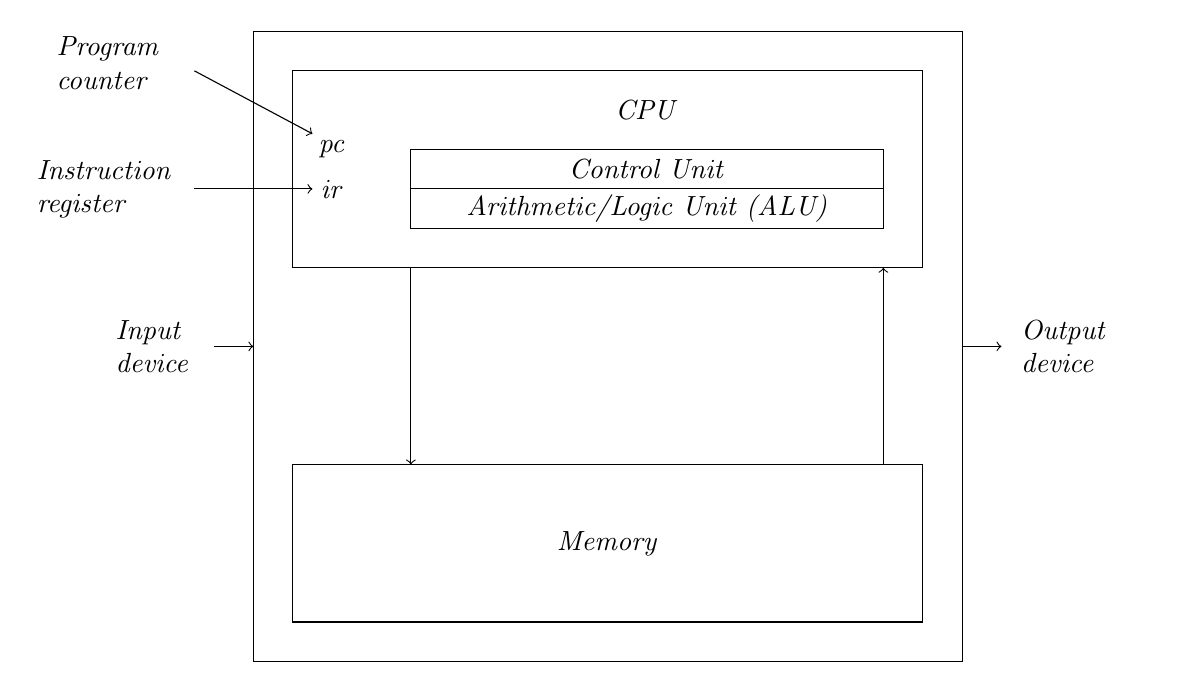
\begin{tikzpicture}
		    \draw (2, 0) rectangle (11, 8);

		    \draw (2.5, 5) rectangle (10.5, 7.5);
		    \node (cpu) at (7, 7) {\textit{CPU}};
		    \node (pc) at (3, 6.5) {\textit{pc}};
		    \node (ir) at (3, 6) {\textit{ir}};
		    \draw (4, 6) rectangle (10, 6.5) node[pos = 0.5]{\textit{Control Unit}};
		    \draw (4, 5.5) rectangle (10, 6) node[pos = 0.5]{\textit{Arithmetic/Logic Unit (ALU)}};

			\draw[->] (4, 5) -- (4, 2.5);
			\draw[<-] (10 , 5) -- (10, 2.5);

		    \draw (2.5, 0.5) rectangle (10.5, 2.5) node[pos = 0.5]{\textit{Memory}};

			\draw[->] (1.5, 4) -- (2, 4);
			\node (inputdevice) at (1, 4) [text width = 1.5cm]{\textit{Input device}};

			\draw[->] (11, 4) -- (11.5, 4);
			\node (outputdevice) at (12.5, 4) [text width = 1.5cm]{\textit{Output device}};

			\draw[->] (1.25, 7.5) -- (2.75, 6.7);
			\node (programcounter) at (0.25, 7.6) [text width = 1.5cm]{\textit{Program counter}};

			\draw[->] (1.25, 6) -- (2.75, 6);
			\node (instructionregister) at (0, 6) [text width = 1.5cm]{\textit{Instruction register}};
		\end{tikzpicture}
		\caption{Von Neumann Architecture.}
		\label{fig:vonneumann}
	\end{figure}
}

\par{
	\begin{figure}[!htb]
		\centering
		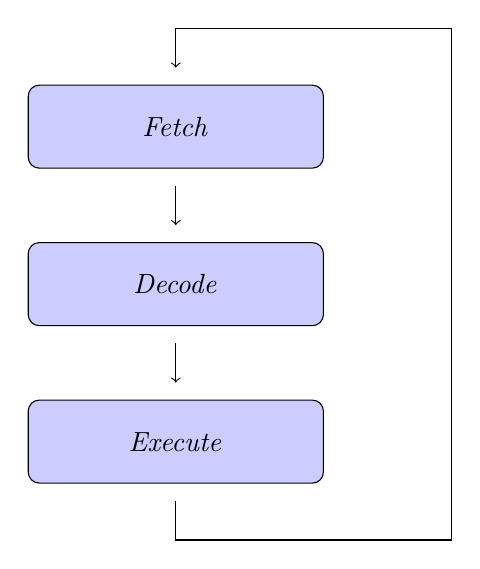
\begin{tikzpicture}
			\node[block] (fetch) at (0, 8) {\textit{Fetch}};
			\draw[->] (0, 7.25) -- (0, 6.75);
			\node[block] (decode) at (0, 6) {\textit{Decode}};
			\draw[->] (0, 5.25) -- (0, 4.75);
			\node[block] (execute) at (0, 4) {\textit{Execute}};
			\draw[->] (0, 3.25) -- (0, 2.75) -- (3.5, 2.75) -- (3.5, 9.25) -- (0, 9.25) -- (0, 8.75);
		\end{tikzpicture}
		\caption{Fetch-Decode-Execute cycle.}
		\label{fig:fetchdecodeexecute}
	\end{figure}
}
\clearpage

\subsection*{DLX Machine}

\par{
	\noindent
	\parskip0pt\begin{itemize}
		\item{Control unit: \newline
			Instruction register (ir) and program counter (pc).
		}
		\item{Arithmetic unit: \newline
			32x 32-bit registers; \texttt{reg[0]}, \texttt{reg[1]}, \ldots, \texttt{reg[31]}. \texttt{reg[0]} always contains the value \texttt{0} and \texttt{reg[31]} is the link register. Both are reserved by convention and must not be used for any other purpose.
		}
		\item{Memory: \newline
			n 32-bit words, byte-addressed (see Figure~\ref{fig:byteaddressedvisualization}), word-aligned; \newline \texttt{mem[0]}, \ldots, \texttt{mem[n - 1]}.
			\begin{figure}[!htb]
				\centering
				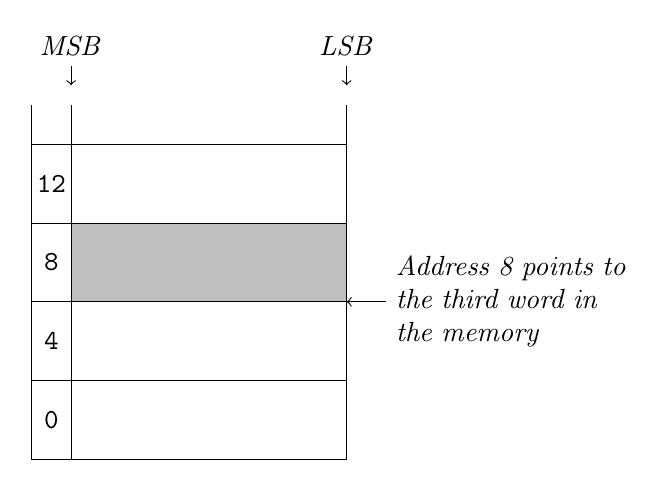
\begin{tikzpicture}
					\draw (0, 4.5) -- (0, 0) -- (4, 0) -- (4, 4.5);
					\draw (0.5, 4.5) -- (0.5, 0);
					\draw (0, 1) -- (4, 1);
					\draw (0, 2) -- (4, 2);
					\draw (0, 3) -- (4, 3);
					\draw (0, 4) -- (4, 4);

					\draw[<-] (0.5, 4.75) -- (0.5, 5) node[above] {\textit{MSB}};
					\draw[<-] (4, 4.75) -- (4, 5) node[above] {\textit{LSB}};
					
					\node at (0.25, 0.5) {\texttt{0}};
					\node at (0.25, 1.5) {\texttt{4}};
					\node at (0.25, 2.5) {\texttt{8}};
					\node at (0.25, 3.5) {\texttt{12}};

					\draw[fill = gray!50] (0.5, 2) rectangle (4, 3);

					\draw[<-] (4, 2) -- (4.5, 2) node[right, text width = 3cm] {\textit{Address 8 points to the third word in the memory}};
				\end{tikzpicture}
				\caption{Visualization of a byte-addressed memory of 32-bit words.}
				\label{fig:byteaddressedvisualization}
			\end{figure}
		}
	\end{itemize}
}

\clearpage

\subsection*{Syntax Formats}

\par{
	\noindent
	General syntax of an instruction: \texttt{op a, b, c}.
}

\subsubsection*{F1}

\par{
	\noindent
	The length of \texttt{a} and \texttt{b} allow to address all 32 registers. The two's complement is used here because the implementation of arithmetics is easier (in contrast to the one's complement).
	\begin{figure}[!htb]
		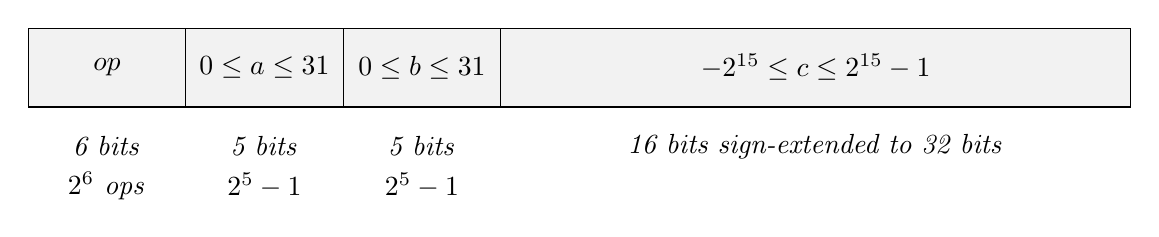
\begin{tikzpicture}
			\draw[fill = gray!10] (0, 1) rectangle (14, 2);
			
			\draw (2, 1) -- (2, 2);
			\node at (1, 1.5) {\texttt{$op$}};
			\node at (1, 0.5) {\textit{6 bits}};
			\node at (1, 0) {\textit{$2^6$ ops}};

			\draw (4, 1) -- (4, 2);
			\node at (3, 1.5) {\texttt{$0 \le a \le 31$}};
			\node at (3, 0.5) {\textit{5 bits}};
			\node at (3, 0) {\textit{$2^5 - 1$}};

			\draw (6, 1) -- (6, 2);
			\node at (5, 1.5) {\texttt{$0 \le b \le 31$}};
			\node at (5, 0.5) {\textit{5 bits}};
			\node at (5, 0) {\textit{$2^5 - 1$}};

			\node at (10, 1.5) {\texttt{$-2^{15} \le c \le 2^{15} - 1$}};
			\node at (10, 0.5) {\textit{16 bits sign-extended to 32 bits}};
		\end{tikzpicture}
	\end{figure}
}

\subsubsection*{F2}

\par{
	\noindent
	E.g. \texttt{R1 = R2 + R3}
	\begin{figure}[!htb]
		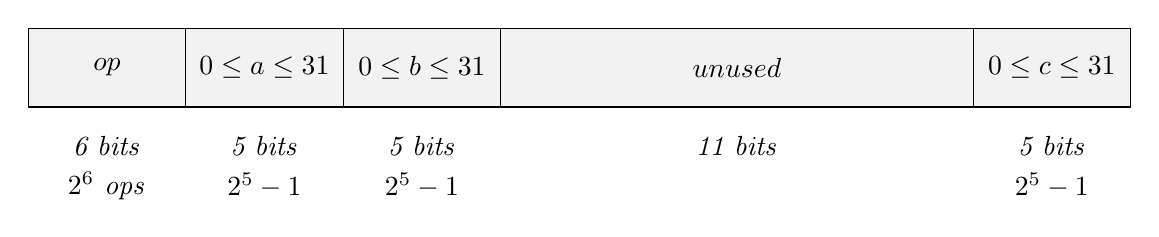
\begin{tikzpicture}
			\draw[fill = gray!10] (0, 1) rectangle (14, 2);
			
			\draw (2, 1) -- (2, 2);
			\node at (1, 1.5) {\texttt{$op$}};
			\node at (1, 0.5) {\textit{6 bits}};
			\node at (1, 0) {\textit{$2^6$ ops}};

			\draw (4, 1) -- (4, 2);
			\node at (3, 1.5) {\texttt{$0 \le a \le 31$}};
			\node at (3, 0.5) {\textit{5 bits}};
			\node at (3, 0) {\textit{$2^5 - 1$}};

			\draw (6, 1) -- (6, 2);
			\node at (5, 1.5) {\texttt{$0 \le b \le 31$}};
			\node at (5, 0.5) {\textit{5 bits}};
			\node at (5, 0) {\textit{$2^5 - 1$}};

			\draw (12, 1) -- (12, 2);
			\node at (9, 1.5) {\texttt{$unused$}};
			\node at (9, 0.5) {\textit{11 bits}};

			\node at (13, 1.5) {\texttt{$0 \le c \le 31$}};
			\node at (13, 0.5) {\textit{5 bits}};
			\node at (13, 0) {\textit{$2^5 - 1$}};
		\end{tikzpicture}
	\end{figure}
}

\subsubsection*{F3}

\par{
	\noindent
	Absolute addressing in memory.
	\begin{figure}[!htb]
		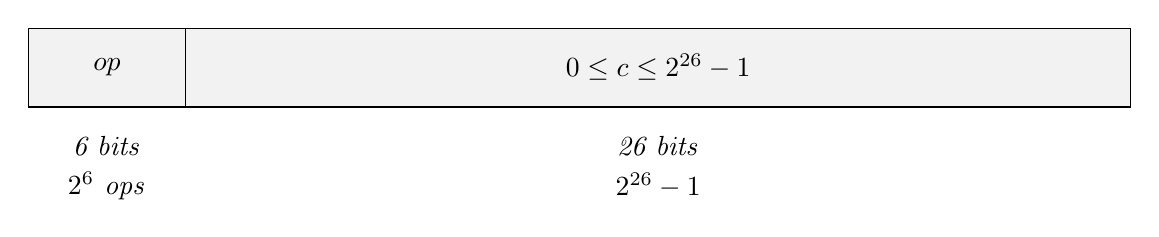
\begin{tikzpicture}
			\draw[fill = gray!10] (0, 1) rectangle (14, 2);
			
			\draw (2, 1) -- (2, 2);
			\node at (1, 1.5) {\texttt{$op$}};
			\node at (1, 0.5) {\textit{6 bits}};
			\node at (1, 0) {\textit{$2^6$ ops}};

			\node at (8, 1.5) {\texttt{$0 \le c \le 2^{26} - 1$}};
			\node at (8, 0.5) {\textit{26 bits}};
			\node at (8, 0) {\textit{$2^{26} - 1$}};
		\end{tikzpicture}
	\end{figure}
}

\par{
	\noindent
	\underline{Von Neumann Bottleneck:}	Memory read/write operations limit the performance.	
}

\clearpage

\subsection*{Register Instructions}

\subsubsection*{Arithmetic Instructions}

\par{
    \noindent
    \textbf{F1}
}

\par{
    \noindent
    \begin{tabular}{llll}
        \hline
        Instruction 			& Semantics 							& Additional information 								\\
        \hline
        \hline
        \texttt{ADDI a, b, c}   &   \texttt{reg[a]:=reg[b]+c;}          &   Add immediate                                       \\
                                &   \texttt{pc:=pc+4;}                  &   \texttt{c} is data (a constant)                     \\
        \texttt{SUBI a, b, c}   &   \texttt{reg[a]:=reg[b]-c;}          &   Substract immediate                                 \\
                                &   \texttt{pc:=pc+4;}                  &   \texttt{c} is data (a constant)                     \\
        \texttt{MULI a, b, c}   &   \texttt{reg[a]:=reg[b]*c;}          &   Multiply immediate                                  \\
                                &   \texttt{pc:=pc+4;}                  &   \texttt{c} is data (a constant)                     \\
        \texttt{DIVI a, b, c}   &   \texttt{reg[a]:=reg[b]/c;}          &   Divide immediate                                    \\
                                &   \texttt{pc:=pc+4;}                  &   \texttt{c} is data (a constant)                     \\
        \texttt{MODI a, b, c}   &   \texttt{reg[a]:=reg[b]\%c;}         &   Modulo immediate                                    \\
                                &   \texttt{pc:=pc+4;}                  &   \texttt{c} is data (a constant)                     \\
        \texttt{CMPI a, b, c}   &   \texttt{reg[a]:=reg[b]-c;}          &   Compare immediate                                   \\
                                &   \texttt{pc:=pc+4;}                  &   \texttt{c} is data (a constant)                     \\
                                &                                       &   \texttt{reg[a]==0 \textbf{if} reg[b]==c}            \\
                                &                                       &   \texttt{reg[a]>=0 \textbf{if} reg[b]>=c}            \\
                                &                                       &   \texttt{reg[a]>0 \textbf{if} reg[b]>c}              \\
                                &                                       &   \texttt{reg[a]=<0 \textbf{if} reg[b]=<c}            \\
                                &                                       &   \texttt{reg[a]<0 \textbf{if} reg[b]<c}              \\
                                &                                       &   \texttt{reg[a]!=0 \textbf{if} reg[b]!=c}            \\
        \hline
    \end{tabular}
}
\clearpage

\par{
    \noindent
    \textbf{F2}
}

\par{
    \noindent
    \begin{tabular}{llll}
        \hline
        Instruction 			& Semantics 							& Additional information 								\\
        \hline
        \hline
        \texttt{ADD a, b, c}    &   \texttt{reg[a]:=reg[b]+reg[c];}     &   Add                                                 \\
                                &   \texttt{pc:=pc+4;}                  &   Register addressing \texttt{reg[c]}                 \\
        \texttt{SUB a, b, c}    &   \texttt{reg[a]:=reg[b]-reg[c];}     &   Substract                                           \\
                                &   \texttt{pc:=pc+4;}                  &   Register addressing \texttt{reg[c]}                 \\
        \texttt{MUL a, b, c}    &   \texttt{reg[a]:=reg[b]*reg[c];}     &   Multiply                                            \\
                                &   \texttt{pc:=pc+4;}                  &   Register addressing \texttt{reg[c]}                 \\
        \texttt{DIV a, b, c}    &   \texttt{reg[a]:=reg[b]/reg[c];}     &   Divide                                              \\
                                &   \texttt{pc:=pc+4;}                  &   Register addressing \texttt{reg[c]}                 \\
        \texttt{MOD a, b, c}    &   \texttt{reg[a]:=reg[b]\%reg[c];}    &   Modulo                                              \\
                                &   \texttt{pc:=pc+4;}                  &   Register addressing \texttt{reg[c]}                 \\
        \texttt{CMP a, b, c}    &   \texttt{reg[a]:=reg[b]-reg[c];}     &   Compare                                             \\
                                &   \texttt{pc:=pc+4;}                  &   Register addressing \texttt{reg[c]}                 \\
                                &                                       &   \texttt{reg[a]==0 \textbf{if} reg[b]==reg[c]}       \\
                                &                                       &   \texttt{reg[a]>=0 \textbf{if} reg[b]>=reg[c]}       \\
                                &                                       &   \texttt{reg[a]>0 \textbf{if} reg[b]>reg[c]}         \\
                                &                                       &   \texttt{reg[a]=<0 \textbf{if} reg[b]=<reg[c]}       \\
                                &                                       &   \texttt{reg[a]<0 \textbf{if} reg[b]<reg[c]}         \\
                                &                                       &   \texttt{reg[a]!=0 \textbf{if} reg[b]!=reg[c]}       \\
        \hline
    \end{tabular}   
}

\subsubsection*{Register Allocation Problem}

\par{
    \noindent
    Registers have to be used in order to execute an instruction. There are 29 registers (in theory) to use. In practice, at least in this course, less registers can be used because some registers are reserved for special purposes (stack pointer, heap pointer, globals pointer, frame pointer, \ldots). It must be guaranteed that these will not be used and furthermore already allocated registers must not be used for an instruction.
}
\clearpage

\par{
    \noindent
    \underline{Examples:}
    \par{
        \noindent
        \begin{tabular}{lll}
            \hline
            C Code                  &   Instructions                &    Additional information                             \\
            \hline
            \hline
            \rowcolor{blue!25}                
            \texttt{1 + 2;}         &   \texttt{ADDI 1, 0, 1}       &   First, naive solution                               \\
            \rowcolor{blue!25}
                                    &   \texttt{ADDI 2, 0, 2}       &                                                       \\
            \rowcolor{blue!25}
                                    &   \texttt{ADD 1, 1, 2}        &                                                       \\
            \rowcolor{green!25}
            \texttt{1 + 2;}         &   \texttt{ADDI 1, 0, 1}       &   Second, better solution                             \\
            \rowcolor{green!25}
                                    &   \texttt{ADDI 1, 1, 2}       &                                                       \\
            \rowcolor{red!25}
            \texttt{1 + 2;}         &   \texttt{ADDI 1, 0, 3}       &   Third, best solution                                \\
            \rowcolor{red!25}
                                    &                               &   Constant folding                                    \\   
            \hline
            \texttt{if(1 < 2)}      &   \texttt{ADDI 1, 0, 1}       &                                                       \\
                                    &   \texttt{ADDI 2, 0, 2}       &                                                       \\
                                    &   \texttt{CMP 1, 0, 2}        &                                                       \\
                                    &   \texttt{BGE 1, 0, <loc>}    &  \texttt{<loc>} represents the line of code in the    \\
                                    &                               &   assembly code the CPU continues with                \\
            \hline
        \end{tabular}
    }    
}

\subsection*{Memory Instructions}

\par{
    \noindent
    \textbf{F1}
}

\par{
    \noindent
    \begin{tabular}{llll}
        \hline
        Instruction 			& Semantics 							& Additional information 								\\
        \hline
        \hline
        \texttt{LDW a, b, c}    &   \texttt{reg[a]:=mem[(reg[b]+c)/4];} &   Load word (from memory)                             \\
                                &   \texttt{pc:=pc+4;}                  &   Register-relative addressing                        \\
        \texttt{STW a, b, c}    &   \texttt{mem[(reg[b]+c)/4]:=reg[a];} &   Store word (into memory)                            \\
                                &   \texttt{pc:=pc+4;}                  &   Register-relative addressing                        \\
        \texttt{POP a, b, c}    &   \texttt{reg[a]:=mem[reg[b]/4];}     &   Pop (from stack)                                    \\
                                &   \texttt{reg[b]:=reg[b]+c;}          &   \texttt{c}: size of the popped chunk                \\
                                &   \texttt{pc:=pc+4;}                  &   \texttt{reg[b]}: contains stack pointer             \\
        \texttt{PSH a, b, c}    &   \texttt{reg[b]:=reg[b]-c;}          &   Push (onto stack)                                   \\
                                &   \texttt{mem[reg[b]/4]:=reg[a];}     &   \texttt{c}: size of the popped chunk                \\
                                &   \texttt{pc:=pc+4;}                  &   \texttt{reg[b]}: contains stack pointer             \\
        \hline
    \end{tabular}   
}

\par{
    \noindent
    The stack grows from high to low addresses (top-down). In the \texttt{POP} and \texttt{PSH} instructions, \texttt{reg[b]:=reg[b]+c} and \texttt{reg[b]:=reg[b]-c} represent the actual removal of the element from the stack, respectively. In case of the C* language \texttt{c} will always be \texttt{4} because only a single type (\textbf{\texttt{int}}) exists in this particular language. In general \texttt{c} is the amount of data you want to remove from the stack.
}

\par{
    \noindent
    Without register-relative addressing, which is a concrete form of indirect addressing, you could only talk about as many memory cells as your program uses. The only way to get the same expressivity as with register-relative addressing is to write self-modifying code.
}
\clearpage

\par{
    \begin{figure}[!htb]
        \centering
        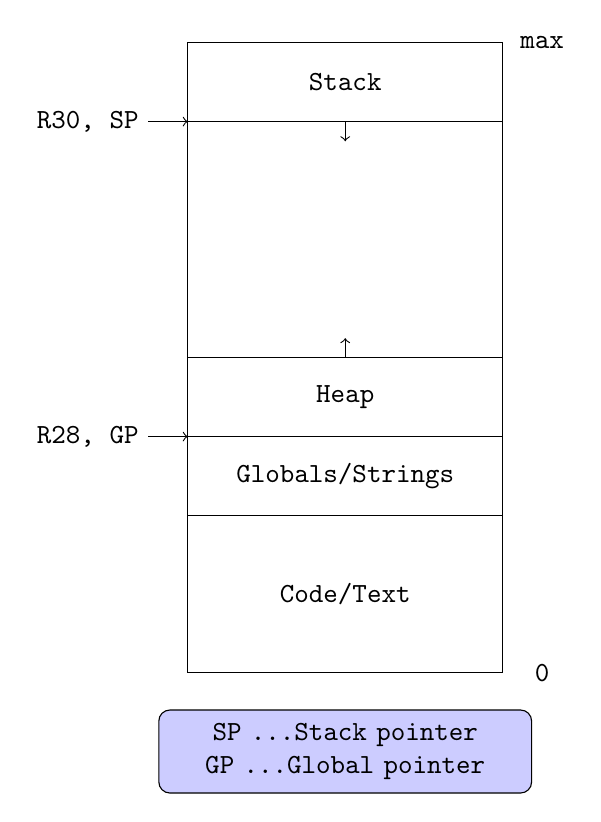
\begin{tikzpicture}
            \draw (2, 1.5) rectangle (6, 9.5);
            
            \node at (6.5, 1.5) {\texttt{0}};
            \node at (6.5, 9.5) {\texttt{max}};

            \draw (2, 8.5) -- (6, 8.5);
            \node at (4, 9) {\texttt{Stack}};
            \draw[->] (4, 8.5) -- (4, 8.25);

            \draw (2, 3.5) -- (6, 3.5);
            \node at (4, 2.5) {\texttt{Code/Text}};
            
            \draw (2, 4.5) -- (6, 4.5);
            \node at (4, 4) {\texttt{Globals/Strings}};

            \draw (2, 5.5) -- (6, 5.5);
            \node at (4, 5) {\texttt{Heap}};
            \draw[->] (4, 5.5) -- (4, 5.75);

            \draw[<-] (2, 8.5) -- (1.5, 8.5) node[left]{\texttt{R30, SP}};
            \draw[<-] (2, 4.5) -- (1.5, 4.5) node[left]{\texttt{R28, GP}};

			

            \node[block] at (4, 0.5) [text width = 4.5cm]{\texttt{SP \ldots Stack pointer GP \ldots Global pointer}};
        \end{tikzpicture}
        \caption{Memory layout when executing a program}
        \label{fig:memorylayout}
    \end{figure}
}

\par{
    \noindent
    \underline{Examples:}
    \par{
        \noindent
        \begin{tabular}{lll}
            \hline
            C Code                  &   Instructions                &    Additional information                         			\\
            \hline
            \hline
            \rowcolor{blue!25}                
            \texttt{int x;}         &   \texttt{LDW 1, 28, -4}      &   \texttt{R1 := x}                               				\\
            \rowcolor{blue!25}
            \texttt{x = x + 1;}		&   \texttt{ADDI 2, 0, 1}       &   \texttt{R2 := 1}                                            \\
            \rowcolor{blue!25}
                                    &   \texttt{ADD 1, 1, 2}        &   \texttt{R1 := R1 + R2}                                    	\\
			\rowcolor{blue!25}
                                    &   \texttt{STW 1, 28, -4}      &   \texttt{mem[x] = R1}                                       	\\
            \rowcolor{green!25}
            \texttt{*x + 1;}        &   \texttt{LDW 1, 28, -4}      &   \texttt{R1 := x}                             				\\
            \rowcolor{green!25}
                                    &   \texttt{LDW 1, 1, 0}       	&   \texttt{R1 := mem[R1 + 0]}                               	\\
			\rowcolor{green!25}
                                    &   \texttt{ADDI 2, 0, 1}       &   \texttt{R2 := 1}                                        	\\
			\rowcolor{green!25}
                                    &   \texttt{ADD 1, 1, 2}       	&	\texttt{R1 := R1 + R2}                   					\\
            \rowcolor{red!25}
            \texttt{*(x + 1);}     	&   \texttt{LDW 1, 28, -4}      &   \texttt{R1 := x}                                			\\
            \rowcolor{red!25}
                                    &   \texttt{ADDI 2, 0, 4} 		&   \texttt{R2 := 0 + 4}, (4 because it's an address)			\\   
			\rowcolor{red!25}
                                    &   \texttt{ADD 1, 1, 2} 		&   \texttt{R1 := R1 + R2}										\\
			\rowcolor{red!25}
                                    &   \texttt{LDW 1, 1, 0} 		&   \texttt{R1 := mem[R1 + 0]}           						\\
			\rowcolor{red!25}
									&								&	\texttt{*(x + i)} is equivalent to \texttt{x[i]}			\\
            \hline
        \end{tabular}
    }    
}

\par{
	\noindent
	When dealing with \texttt{*(x + 1)}, the type of \texttt{x} has to be known as well as its size in the memory. The size of \texttt{x} in the memory determines the offset which is added to the address of \texttt{x}. In case of the C* language this value is always \texttt{4} because there is only one type and no support for composed types (\texttt{struct}). Nevertheless, the size of the type needs to be added in general. \newline
	Formula to compute \texttt{*(x + i) = x[i]}: \texttt{x} + \texttt{\textbf{sizeof}(x)} * \texttt{i}.
}

\subsection*{Control Instructions}

\par{
    \noindent
    \textbf{F1}
}

\par{
    \noindent
    \begin{tabular}{llll}
        \hline
        Instruction 			& Semantics 							& Additional information 								\\
        \hline
        \hline
        \texttt{BEQ a, c}    	&   \texttt{if(reg[a]==0) pc:=pc+c*4;} 	&   Branch on equal to zero                            	\\
                                &   \texttt{else pc:=pc+4;}             &  	Conditional branch, pc-relative						\\
        \texttt{BGE a, c}    	&   \texttt{if(reg[a]>=0) pc:=pc+c*4;} 	&   Branch on greater than or equal to zero             \\
                                &   \texttt{else pc:=pc+4;}             &  	Conditional branch, pc-relative						\\
        \texttt{BGT a, c}    	&   \texttt{if(reg[a]>0) pc:=pc+c*4;} 	&   Branch on greater than to zero                      \\
                                &   \texttt{else pc:=pc+4;}             &  	Conditional branch, pc-relative						\\
        \texttt{BLE a, c}    	&   \texttt{if(reg[a]<=0) pc:=pc+c*4;} 	&   Branch on less than or equal to zero                \\
                                &   \texttt{else pc:=pc+4;}             &  	Conditional branch, pc-relative						\\
		\texttt{BLT a, c}    	&   \texttt{if(reg[a]<0) pc:=pc+c*4;} 	&   Branch on less than to zero                        	\\
                                &   \texttt{else pc:=pc+4;}             &  	Conditional branch, pc-relative						\\
        \texttt{BNE a, c}    	&   \texttt{if(reg[a]!=0) pc:=pc+c*4;} 	&   Branch on not equal to zero                         \\
                                &   \texttt{else pc:=pc+4;}             &  	Conditional branch, pc-relative						\\
        \texttt{BR c}    		&   \texttt{pc:=pc+c*4;} 				&   Branch (unconditional)								\\
        \texttt{BSR c}    		&   \texttt{reg[31]:=pc+4;} 			&   Branch to subroutine (unconditional)                \\
                                &   \texttt{pc:=pc+c*4;}             	&  	Tthe link register (\texttt{R31}) is saved to be	\\
								&										&	able to return to the correct instruction			\\
        \hline
    \end{tabular}   
}

\par{
    \noindent
    \textbf{F2}
}

\par{
    \noindent
    \begin{tabular}{llll}
        \hline
        Instruction 	& Semantics 				& Additional information		\\
        \hline
        \hline
        \texttt{RET c}	&   \texttt{pc:=reg[c];}	&	\texttt{c} = \texttt{R31}	\\
        \hline
    \end{tabular}   
}

\par{
    \noindent
    \textbf{F3}
}

\par{
    \noindent
    \begin{tabular}{llll}
        \hline
        Instruction 	& Semantics 				& Additional information		\\
        \hline
        \hline
        \texttt{JSR c}	&   \texttt{reg[31]:=pc+4;}	&	\texttt{c} = \texttt{R31}	\\
						&	\texttt{pc:=c;}			&	absolute addressing			\\
        \hline
    \end{tabular}   
}

\par{
	\noindent
	All branches (conditional as well as unconditional) are pc-relative. The multiplication of \texttt{c} by \texttt{4} is because the words in the memory are byte-addressed. Branches are useful (especially because they operate pc-relative) because you generate so-called \textit{relocatable code}. \textit{Relocatable code} can be moved in memory anywhere and will not change its behavior because every address is computed relative to the program counter. The drawback of branches is the restriction of the addressable space: there may be more memory than you can use with branches. The solution is absolute addressing used by the F3 format. The F3 format allows you to address a range of $2^{26}$.
}
